\documentclass[12pt]{article}
\usepackage{enumerate}
\usepackage{notes}

\newcommand{\LHS}{\text{LHS}}
\newcommand{\RHS}{\text{RHS}}

\begin{document}
\title{Introduction to University Mathematics}
\maketitle

\section*{Sheet 1}
\subsection*{} % 1
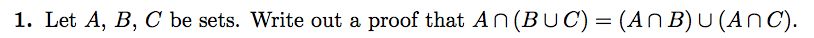
\includegraphics[width=400pt]{img/iulm-1-1.png}
\begin{mdframed}

Take the following things to have been defined already: intersection, union, subset.

Define $\LHS := A \cap (B \cup C)$ and $\RHS := (A \cap B) \cup (A \cap C)$.

We have to prove
\begin{enumerate}
\item that $\LHS \subset \RHS$, and
\item that $\RHS \subset \LHS$.
\end{enumerate}

\subsubsection*{Proof of (1)}
If $\LHS = \emptyset$, then (1) is true.

Alternatively, suppose $\LHS \neq \emptyset$ and let $x \in \LHS$. Then by the
definition of intersection, $x \in A$ and $x \in B \cup C$, and therefore by
the definition of union either $x \in B$ or $x \in C$.

Suppose $x \in B$. Then we have $x \in A$ and $x \in B$, so by the definition
of intersection $x \in A \cap B$. The RHS is the union of two sets, of which
$A \cap B$ is one. Therefore by the definition of union $x \in \RHS$.

Alternatively we can suppose $x \in C$. Since union and intersection commute,
$B$ and $C$ play equivalent roles and $x \in C$ leads to the same conclusion
that $x \in \RHS$ by an analogous argument to that above.

Therefore $\LHS \subset \RHS$.

\subsubsection*{Proof of (2)}
If $\RHS = \emptyset$, then (2) is true.

Alternatively, suppose $\RHS \neq \emptyset$ and let $x \in \RHS$. Then by the
definition of union, $x \in A \cap B$ or $x \in A \cap C$. Suppose
$x \in A \cap B$ (and label this ``supposition 1''). Then $x \in A$ and
$x \in B$. $x \in B \implies x \in B \cup Z$ for any set $Z$, so
$x \in B \cup C$, and therefore $x \in \LHS$.

Alternatively, at supposition 1, we could suppose $x \in A \cap C$. Due to
the symmetry resulting from commutativity of union and intersection, this also
leads to the conclusion $x \in \LHS$ by an identical argument.

Therefore $\RHS \subset \LHS$. \qed
\end{mdframed}


\subsection*{} % 2
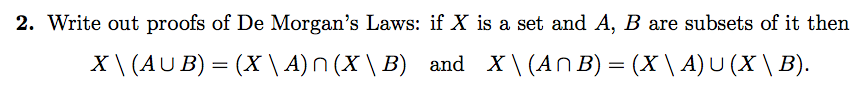
\includegraphics[width=400pt]{img/iulm-1-2.png}
\begin{mdframed}
\end{mdframed}

\newpage
\subsection*{} % 3
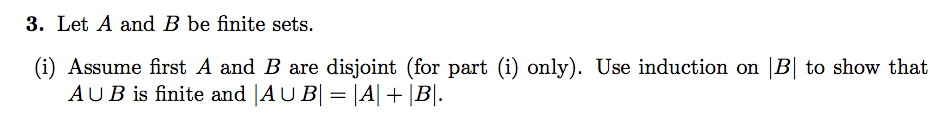
\includegraphics[width=400pt]{img/iulm-1-3.png}
\begin{mdframed}
First, observe that a set $X$ is finite if and only if $|X| \in \N$.

Second, observe that, if $|A \cup B| = |A| + |B|$ with $A$ and $B$ finite, then
$A \cup B$ is finite. Therefore it will suffice to show that
$|A \cup B| = |A| + |B|$.

We are told that $A$ and $B$ are finite.

Suppose $|B| = 0$. Then $B = \emptyset$ and $|A \cup B| = |A| = |A| + |B|$ as required.

Now suppose the desired result holds whenever $|B| = n$, i.e.
$|A \cup B| = |A| + n$. Specifically, let $B = X$ with $|X| = n$. We want to
show that when $|B|$ is increased to $n+1$, then $|A \cup B| = |A| + n+1$.

To increase $|B|$ to $n+1$, a new element $y \notin X$ must be added to
$B$.\footnote{I'm not comfortable with this. When passing from $|B| = n$ to
  $|B| = n+1$, the two sets need not differ just by adjoining a new element;
  they might be completely different, with no elements in
  common. \label{cardinality-induction-discomfort}} Also $y \notin A$ since we
are told that $A$ and $B$ are disjoint. So now
\begin{align*}
  |A \cup B| &= |A \cup (X \cup \{y\})|\\
             &= |(A \cup X) \cup \{y\}| ~~~~\text{by associativity of union operation.}
\end{align*}
And since $y \notin X$ and $y \notin A$, $|(A \cup X) \cup \{y\}| = |A \cup X| + 1 = n + 1$.

Therefore by induction,
\begin{align*}
  |A \cup B| = |A| + |B|
\end{align*}
for finite and disjoint $A$, $B$. \qed
\end{mdframed}

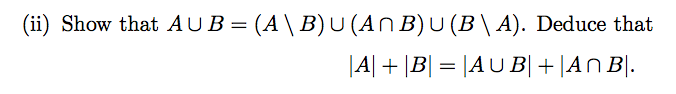
\includegraphics[width=300pt]{img/iulm-1-3-ii.png}
\begin{mdframed}

First, we show that
\begin{align}
  A \cup B ~~~ &\subset ~~~ (A \setminus B) \cup (A \cap B) \cup (B \setminus A).\label{3-forward}
\end{align}
Let $\LHS$ and $\RHS$ denote the expressions on the left- and right-hand sides
of the subset operator, respectively.

To show \eqref{3-forward}, first note that if $A \cup B = \emptyset$ then
\eqref{3-forward} is true. Alternatively suppose $A \cup B \neq \emptyset$ and
let $x \in A \cup B$. Note that since union and intersection commute, there are
symmetries in LHS and RHS, and in fact $A$ and $B$ are
exchangeable\footnote{need to define ``exchangeable''} in those
expressions. With that in mind, suppose that $x \in A$. Then either
$x \in A \cap B$ or $x \in A \setminus B$. So $x$ belongs to one of the three
sets in the union on the RHS. Alternatively we could have chosen $x \in B$, but
due to the symmetry described above we would be able to make an analogous
argument to conclude again that $x \in \RHS$. Thus we've shown that either LHS
is empty, or that any element of LHS is also an element of RHS, proving
\eqref{3-forward}.

Next we show that
\begin{align}
  (A \setminus B) \cup (A \cap B) \cup (B \setminus A) ~~~ &\subset ~~~ A \cup B. \label{3-backward}
\end{align}

Again, let $\LHS$ and $\RHS$ denote the expressions on the left- and right-hand
sides of the subset operator, respectively.

And again, if $\LHS = \emptyset$ then \eqref{3-backward} is
true. Alternatively, suppose $\LHS \neq \emptyset$. This implies that either
$A$ or $B$ is non-empty, since at least one of them has contributed at least
one element to the union. Suppose that $A \neq \emptyset$ and let $x \in
A$. Then $x \in A \cup B = \RHS$. Alternatively we could have chosen
$B \neq \emptyset$ and reached the same conclusion. Thus we've shown that
either LHS is empty, or that any element of LHS is also an element of RHS,
proving \eqref{3-backward}, and completing the proof of equality of LHS and
RHS.

Finally we are asked to deduce that $|A| + |B| = |A \cup B| + |A \cap B|$, or
equivalently $|A \cup B| = |A| + |B| - |A \cap B|$. From the above, we know
that
\begin{align*}
  |A \cup B| &= |(A \setminus B) \cup (A \cap B) \cup (B \setminus A)|\\
             &= |(A \setminus B)| + |(A \cap B)| + |(B \setminus A)|,
\end{align*}
since the 3 sets are disjoint and union is associative. Now
$|X \setminus Y| = |X| - |X \cap Y|$\footnote{Does this need proof?}, therefore
\begin{align*}
  |A \cup B| &= |A| - |A \cap B| + |(A \cap B)| + |B| - |B \cap A|\\
             &= |A| + |B| - |A \cap B|.
\end{align*}
\qed
\end{mdframed}

\newpage
\subsection*{} % 4
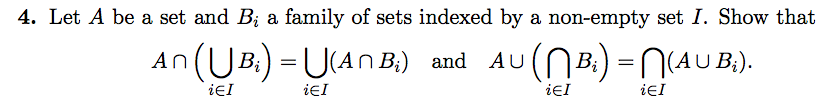
\includegraphics[width=500pt]{img/iulm-1-4.png}
\begin{mdframed}
  \textit{Remark}: these propositions are extensions to the n-ary cases of the
  basic theorems concerning distribution of union over binary intersection, and
  of intersection over binary union. The proofs are by induction on $|I|$,
  relying on the binary base cases.

Let $\alpha \in I$.

The first proposition is $A \cap \bigcup_{i \in I} B_i = \bigcup_{i \in I} (A \cap B_i)$.

If $|I| = 1$ then the result holds since the LHS is
\begin{align*}
  A \cap \bigcap_{i \in \{\alpha\}} B_i = A \cap B_\alpha,
\end{align*}
and the RHS is
\begin{align*}
  \bigcup_{i \in \{\alpha\}} (A \cap B_i) = A \cap B_\alpha.
\end{align*}

For induction, we assume that the proposition holds for $|I| = n \in \N$ and we
seek to show that it holds for $|I| = n + 1$. Specifically, assume it holds
for $I=X$ where $|X| = n$ and consider $I = X \cup \{y\}$ where
$y \notin X$.\footnote{Again, not comfortable with this, see previous footnote
  \ref{cardinality-induction-discomfort}.} Then the LHS is
\begin{align*}
  A \cap \bigcup_{i \in X \cup \{y\}} B_i
  &= A \cap \(\(\bigcup_{i \in X} B_i\) \cup B_y\)\\
  &= \(A \cap \bigcup_{i \in X} B_i\) \cup \(A \cap B_y\) ~~~\text{(distribution of intersection over binary union)}\\
  &= \(\bigcup_{i \in X} (A \cap B_i)\) \cup \(A \cap B_y\) ~~~\text{(by assumption)}\\
  &= \(\bigcup_{i \in X \cup \{y\}} (A \cap B_i)\),
\end{align*}
as desired. This completes a proof by induction of the first proposition.
\end{mdframed}

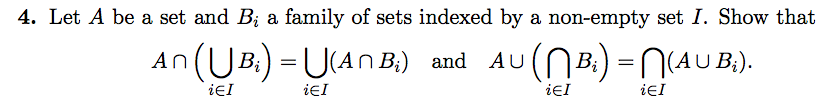
\includegraphics[width=400pt]{img/iulm-1-4.png}
\begin{mdframed}
The second proposition is $A \cup \bigcap_{i \in I} B_i = \bigcap_{i \in I} (A \cup B_i)$.

Let $\alpha \in I$.

If $|I| = 1$ then the result holds since the LHS is
\begin{align*}
  A \cup \bigcap_{i \in \{\alpha\}} B_i = A \cup B_\alpha,
\end{align*}
and the RHS is
\begin{align*}
  \bigcap_{i \in \{\alpha\}} (A \cup B_i) = A \cup B_\alpha.
\end{align*}

For induction, assume that the result holds for $|I| = n > 0$. We seek to show
that it holds for $|I| = n + 1$. Specifically, assume it holds for $I=X$ where
$|X| = n$ and consider $I = Y = X \cup \{y\}$ where $y \notin X$ so that
$|Y| = n + 1$.\footnote{Ditto re. discomfort, see
  \ref{cardinality-induction-discomfort}.} Then the LHS is
\begin{align*}
  A \cup \bigcap_{i \in X \cup \{y\}} B_i
  &= A \cup \(\(\bigcap_{i \in X} B_i\) \cap B_y\)\\
  &= \(A \cup \(\bigcap_{i \in X} B_i\)\) \cap  \(A \cup B_y\) ~~~\text{(distribution of union over binary intersection)}\\
  &= \(\bigcap_{i \in X} (A \cup B_i)\) \cap  \(A \cup B_y\) ~~~\text{(by assumption)}\\
  &= \bigcap_{i \in X \cup \{y\}} (A \cup B_i).
\end{align*}

\end{mdframed}


\newpage
\subsection*{} % 5
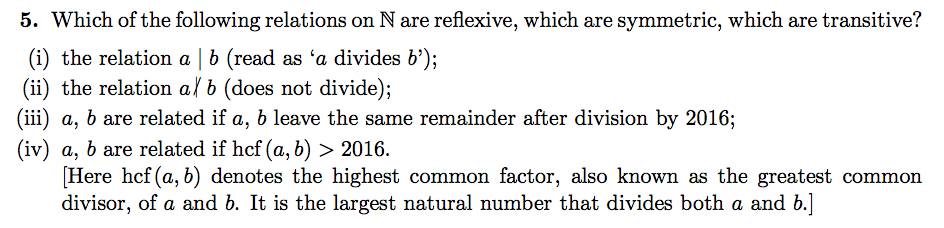
\includegraphics[width=400pt]{img/iulm-1-5.png}
\begin{mdframed}
  \begin{enumerate}[label=(\roman*)]
  \item $a | b$ is reflexive and transitive but not symmetric.
  \item $a \nmid b$ is not reflexive, not symmetric and not transitive (e.g.
    $2 \nmid 3$ and $3 \nmid 4$ yet $2 | 4$.)
  \item The $\mod 2016$ relation is reflexive, symmetric and transitive.
  \item The $\text{hcf} > 2016$ relation is reflexive and symmetric but not
    transitive. (E.g. consider $a = (2016+1), b = 2\cdot(2016+1)\cdot(2016+2)$
    and $c = (2016+2)$. We have $a R b$ and $b R c$ yet not $a R c$.
  \end{enumerate}
\end{mdframed}

\newpage
\subsection*{} % 6
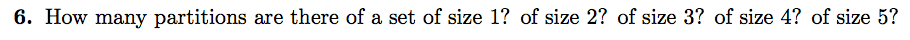
\includegraphics[width=400pt]{img/iulm-1-6.png}
\begin{mdframed}
  Let $P_n$ be the number of partitions of a set of size $n$. It's easy to see
  by direct enumeration that the first 3 values of $P_n$ are
  \\
  \begin{tabular}{c|c}
    $n$ & $P_n$\\
    \hline
    1 & 1\\
    2 & 2 \\
    3 & 5 \\
  \end{tabular}\\
  \\
  $P_4$ is 15 but from that point onwards it's laborious and error-prone to try
  to enumerate them manually.

  A recursive algorithm for enumerating the partitions of a set of size $n$ is
  given below. From the algorithm, we can see that the following recurrence
  relation holds for $n > 1$. Let $A_{n,i}$ be the $i$-th partition of a set of
  size $n$. Then
  \begin{align*}
    P_n = P_{n-1} + \sum_{i=1}^{P_{n-1}}|A_{n-1,i}|.
  \end{align*}
  This gives the following values:\\\\
  \begin{tabular}{c|c|c}
    $n$ & $|A_{n,i}|$ multiplicites& $P_n$\\
    \hline
    1 & $1 \cdot 1$                                     & 1  \\
    2 & $1 \cdot 1 + 2 \cdot 1$                         & 2  \\
    3 & $1 \cdot 1 + 2 \cdot 3 + 3 \cdot 1$             & 5  \\
    4 & $1 \cdot 1 + 2 \cdot 7 + 3 \cdot 6 + 4 \cdot 1$ & 15 \\
    5 & ...                                             & 52 \\
  \end{tabular}\\
  \newpage
  \begin{minted}{python3}
from copy import deepcopy

def partitions(n):
    """
    Return a list of all partitions of the set {1, 2, ..., n}

    A partition is a list of parts.
    A part is a list of elements.
    """
    if n == 0:
        return [[]]
    else:
        _partitions = []
        for partition in partitions(n - 1):

            # For each part of the n-1 partition, create a new
            # partition in which the new element is added to that part
            # and the other parts are unchanged.
            for i in range(len(partition)):
                _partition = deepcopy(partition)
                _partition[i].append(n)
                _partitions.append(_partition)

            # Also create a new partition in which the new element is
            # added as a singleton.
            _partition = deepcopy(partition)
            _partition.append([n])
            _partitions.append(_partition)

        return _partitions
  \end{minted}
\end{mdframed}

\newpage
\subsection*{} % 7
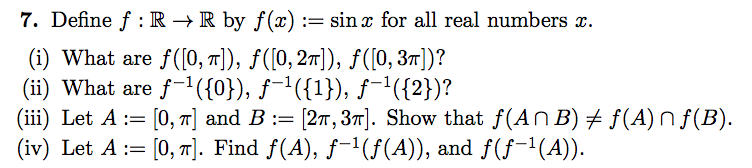
\includegraphics[width=400pt]{img/iulm-1-7.png}
\begin{mdframed}
  \begin{enumerate}[label=(\roman*)]
  \item $f([a,b])$ is the image of the set $[a,b]$ under $f$.
    \begin{itemize}
    \item $f([0, \pi]) = [0, 1]$
    \item $f([0, 2\pi]) = [-1, 1]$
    \item $f([0, 3\pi]) = [-1, 1]$
    \end{itemize}
  \item $f^\1(A)$ is the preimage of $A$ under $f$
    \begin{itemize}
    \item $f^\1(\{0\}) = \{k\pi~|~k \in \Z\}$
    \item $f^\1(\{1\}) = \{\frac{\pi}{2} + 2k\pi ~|~ k \in \Z\}$
    \item $f^\1(\{2\}) = \emptyset$
    \end{itemize}
  \item The LHS is
    \begin{align*}
      f(A \cap B)
      &= f([0, \pi] \cap [2\pi,3\pi])\\
      &= f(\emptyset)\\
      &= \emptyset,
    \end{align*}
    and the RHS is
    \begin{align*}
      f(A) \cap f(B)
      &= f([0, \pi]) \cap f([2\pi,3\pi])\\
      &= [0, 1] \cap [0, 1]\\
      &= [0, 1].
    \end{align*}
  \item
    \begin{itemize}
    \item $f(A) = [0, 1]$
    \item
      \begin{align*}
        f^\1(f(A))
        &= f^\1([0, 1])\\
        &= \bigcup_{k \in \Z} ~[2k\pi, (2k + 1)\pi]
      \end{align*}
    \item
      \begin{align*}
        f(f^\1(A))
        &= f(f^\1([0, \pi]))\\
        &= f(f^\1([0, 1]))\\
        &= f(\bigcup_{k \in \Z} ~[2k\pi, (2k + 1)\pi])\\
        &= [0,1]
      \end{align*}
    \end{itemize}
  \end{enumerate}
\end{mdframed}

\newpage
\subsection*{} % 8
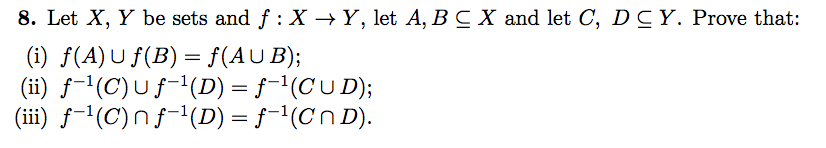
\includegraphics[width=400pt]{img/iulm-1-8.png}
\begin{mdframed}
  \begin{enumerate}[label=(\roman*)]
  \item The claim is that the union of two images is the image of the
    union.

    \textcolor{blue}{This is seeming a bit pedestrian! Is there a more elegant way to do this?}

    First we prove $f(A) \cup f(B) \subset f(A \cup B)$.

    $LHS = \emptyset$ if and only if $A$ and $B$ are both empty (in which case
    $\LHS = f(\emptyset) \cup f(\emptyset) = \emptyset$). In this case, the
    subset relation is true.

    Alternatively, suppose $LHS \neq \emptyset$. This is true if and only if
    $A$ is non-empty or $B$ is non-empty. Suppose $A$ is non-empty and let
    $x \in A$. Then $f(x) \in f(A)$ and so $f(x) \in \LHS$. Also
    $x \in A \cup B$ so $f(x) \in \RHS$. Alternatively, we could have supposed
    $B$ is non-empty, but due to the symmetries in LHS and RHS this would lead
    to the same conclusion. Therefore any element of the LHS is an element of
    the RHS, as required.

    Second, we prove $f(A \cup B) \subset f(A) \cup f(B)$.

    $LHS = \emptyset$ if and only if $A$ and $B$ are both empty (in which case
    $\LHS = f(\emptyset) = \emptyset$). In this case the subset relation is
    true. Alternately assume $A$ is non-empty and let $x \in A$. Then
    $f(x) \in f(A \cup B)$ and $f(x) \in f(A)$, so the element of the LHS is
    contained in the RHS. Alternatively we could have supposed $B$ is
    non-empty, but due to the symmetries in LHS and RHS this would lead to the
    same conclusion. Therefore any element of the LHS is an element of the RHS,
    as required.

  \item Let $\LHS = f^\1(C) \cup f^\1(D)$, and $\RHS = f^\1(C \cup D)$. The
    claim is $LHS=RHS$ (i.e., informally, that the union of preimages is the
    preimage of the union.)

    \textcolor{blue}{Trying a slight variation: contradiction rather than
      proving forwards and reverse subset containment.}

    There are two ways that could be untrue; let's show that they both lead to
    contradictions.
    \begin{enumerate}
    \item There is an element of the LHS which is not an element of the RHS. So
      let $x \in \LHS$ be such an element. Then $f$ maps $x$ into either $C$ or
      $D$. But this would mean that $f$ maps $x$ into $C\cup D$, and therefore
      that $x \in \RHS$, which is a contradiction.
    \item There is an element of RHS which is not an element of LHS. So let $x$
      be such an element. Then $f$ maps $x$ into $C \cup D$. But this means
      that $f$ maps $x$ into either $C$ or $D$, and therefore that
      $x \in \LHS$, which is a contradiction.
    \end{enumerate}
    These contradictions prove that $LHS=RHS$.

  \item Let $LHS = f^\1(C) \cap f^\1(D)$, and $RHS = f^\1(C \cap D)$. The claim
    is that $\LHS = \RHS$ (i.e., informally, that the intersection of preimages
    is the preimage of the intersection).

    There are two ways that could be untrue; let's show that they both lead to
    contradictions.
    \begin{enumerate}
    \item There is an element of the LHS which is not an element of the RHS. So
      let $x \in \LHS$ be such an element. Then $f$ maps $x$ into both $C$ and
      $D$. But then $f$ maps $x$ into $C \cap D$ and therefore $x \in \RHS$,
      which is a contradiction.
    \item There is an element of RHS which is not an element of LHS. So let $x$
      be such an element. Then $f$ maps $x$ into $C \cap D$. But this means
      that $f$ maps $x$ into both $C$ and $D$, and therefore that
      $x \in \LHS$, which is a contradiction.
    \end{enumerate}
    These contradictions prove that $LHS=RHS$.


  \end{enumerate}
\end{mdframed}

\newpage
\subsection*{} % 9
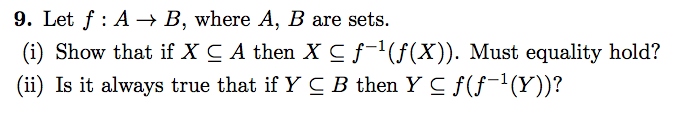
\includegraphics[width=400pt]{img/iulm-1-9.png}
\begin{mdframed}
\begin{enumerate}[label=(\roman*)]
\item The definition of $f^\1(f(X))$ is $\{x~|~f(x) \in f(X)\}$. $X$ is
  certainly a subset of this set, by the definition of $f(X)$. So if we suppose
  an element $x' \in X$ exists for which $x' \notin f^\1(f(X))$, then we have
  an immediate contradiction. Therefore no such $x'$ exists, proving the
  claim.

  No equality does not always hold. As a counter-example, let
  $f: \R \to [-1, 1]$ with $f(x) = \sin(x)$, and let $X = [0,
  \frac{\pi}{2}]$. Then $f(X) = [0, 1]$. However
  $f^\1(f(X)) = \bigcup_{k \in \Z} ~[2k\pi, 2k\pi + \frac{\pi}{2}] \neq X$.
  \textit{Conjecture}: The proposed equality holds if and only if $f$ is
  injective.

\item No, this is not always true. As a counter-example, consider
  $Y \neq \emptyset$ where $Y \cap f(A) = \emptyset$ (i.e. there is no element
  of the domain which is mapped into $Y$ by $f$). Then $f^\1(Y) = \emptyset$
  and so $f(f^\1(Y)) = \emptyset \neq Y$. \textit{Conjecture}: the proposed
  subset relationship holds if and only if $f$ is surjective.
\end{enumerate}
\end{mdframed}

\newpage
\subsection*{} % 10
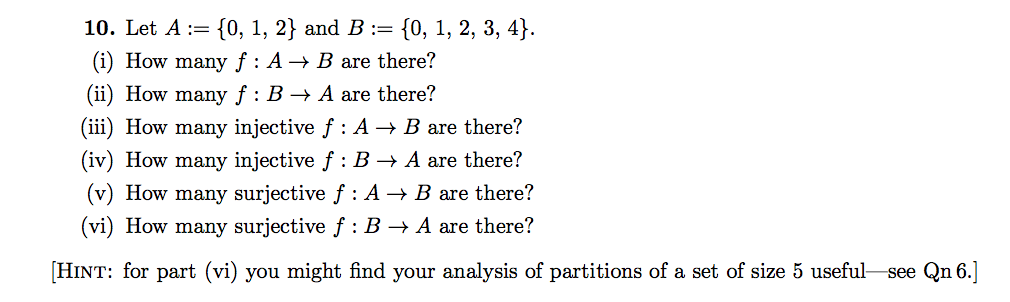
\includegraphics[width=500pt]{img/iulm-1-10.png}
\begin{mdframed}
\begin{enumerate}[label=(\roman*)]

\item The possible values for the domain of $f$ are $\wp(A)$. Let $f_k:A \to B$
  have domain $A^*$ where $|A^*| = k$. For each element $a$ of the domain there
  are $|B| = 5$ possible choices for $f_k(a)$. Therefore there are $|B|^k$ such
  $f_k$ and the total number of $f:A \to B$ is
  \begin{align*}
   \sum_{A^* \in \wp(A)} |B|^{|A^*|}
    = \sum_{k=0}^{|A|} {|A| \choose k} |B|^k
    = \sum_{k=0}^3 {3 \choose k} 5^k
    = 1 \cdot 5^0 % 1 .  1  =   1
    + 3 \cdot 5^1 % 3 .  5  =  15
    + 3 \cdot 5^2 % 3 . 25  =  75
    + 1 \cdot 5^3 % 1 . 125 = 125
    =                         216.
  \end{align*}
\item By the same argument with $A$ and $B$ interchanged, the number of
  $f: B \to A$ is
  \begin{align*}
    \sum_{k=0}^5 {5 \choose k} 3^k
    = 1 \cdot 3^0  % 1 . 1   =   1
    + 5 \cdot 3^1  % 5 . 3   =  15
    + 10 \cdot 3^2 % 10 . 9  =  90
    + 10 \cdot 3^3 % 10 . 27 = 270
    + 5 \cdot 3^4  % 5 . 81  = 405
    + 1 \cdot 3^5  % 1 . 243 = 243
    =                         1024.
  \end{align*}

\item Injective $f:A \to B$ are those $f$ for which each element in the range
  is hit by exactly one element of the domain. Note that the size of the domain
  cannot exceed that of the codomain.

  The possible values for the domain of $f$ are
  $\{A^* ~|~ A^* \in \wp(A), |A^*| \leq |B|\}$. Let $f_k:A \to B$ have domain
  $A^*$ where $|A^*| = k \leq |B|$. Each element of the domain chooses a
  different element of $B$, so the number of $f_k$ is equal to the number of
  ordered subsets of $\{1, 2, \ldots, |B|\}$ of size $k$, which is
  $\frac{|B|!}{(|B| - k)!}$. Therefore the total number of injective
  $f:A \to B$ is
  \begin{align*}
   \sum_{A^* \in \wp(A), |A^*| \leq |B|} \frac{|B|!}{\(|B| - |A^*|\)!}
    &= \sum_{k=0}^{\min(|A|, |B|)} {|A| \choose k} \frac{|B|!}{\(|B| - k\)!}\\
    &= |A|!|B|!\sum_{k=0}^{\min(|A|, |B|)} \frac{1}{k!(|A| - k)! (|B| - k)!}\\
    &= 6 \cdot 120\(\frac{1}{1 \cdot 6 \cdot 120}  % 0
                   +\frac{1}{1 \cdot 2 \cdot 24}   % 1
                   +\frac{1}{2 \cdot 1 \cdot 6}    % 2
                   +\frac{1}{6 \cdot 1 \cdot 2}\)\\  % 3
    &=              1     % 0
                   +15    % 1
                   +60    % 2
                   +60    % 3
     = 136.
  \end{align*}

\item The number of injective $f:B \to A$ is also 136 (the expression above is
  symmetric in $A$ and $B$).

\item Surjective $f:A \to B$ are those $f$ which hit every element of the
  codomain. Therefore the size of the codomain cannot exceed that of the
  domain. Therefore there are no such $f$, since $|A| < |B|$.

\item Let $f_k:B \to A$ have domain $B^*$ where $|B^*| = k \geq |A|$. Each
  element of the domain chooses a different element of $A$, but we also require
  that every element of $A$ is chosen at least once. To count the number of
  ways of doing this, we demand that $|A|$ elements of the domain choose
  distinct values of $A$: there are $|A|!$ ways of making those
  assignments. The remaining $k - |A|$ elements of the domain can choose freely
  from among $A$, so the total number of valid arrangements is
  $|A|!(k - |A|)|A| / k!$, where the factor of $k!$ eliminates duplicates
  differing only in order. Therefore the number of surjective $f:B \to A$ is
  \begin{align*}
    \sum_{B^* \in \wp(B), |B^*| \geq |A|} \frac{|A|!(|B^*| - |A|)|A|}{|B^*|!}
    &= \sum_{k=|A|}^{|B|}{|B| \choose k} \frac{|A|!(k - |A|)|A|}{k!}\\
    &= |B|!|A|!|A|\sum_{k=|A|}^{|B|}\frac{(k - |A|)}{(k!)^2(|B|-k)!}\\
    &= 120 \cdot 6 \cdot 3\(
                \frac{0}{36 \cdot 2}  % 3
              + \frac{1}{24^2 \cdot 1}  % 4
              + \frac{2}{120^2 \cdot 1}  % 5
      \)
    &= \frac{90}{24} + \frac{36}{120}
  \end{align*}


\end{enumerate}
\end{mdframed}

\newpage
\section*{Sheet 2}
\subsection*{}
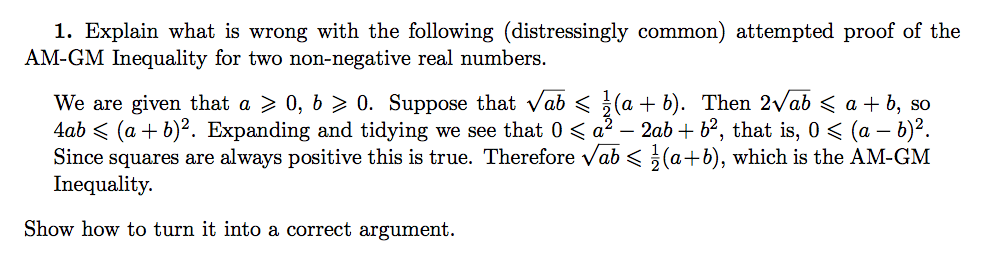
\includegraphics[width=450pt]{img/iulm-2-1.png}
\begin{mdframed}
  The attempted proof is flawed because it has the following form:
  \begin{enumerate}
  \item Suppose [the thing we are trying to prove]
  \item Deduce from this a tautology
  \item Conclude that [the thing we are trying to prove] is true.
  \end{enumerate}
  The problem is that it is possible to deduce a tautology from a false
  statement. For example $-1 = 1 \implies 1 = 1$ by squaring both sides.

  A correct proof follows.

  We are given that $a \geq 0, b \geq 0$. We start by noting that
  $0 \leq (a - b)^2$ is a tautology (true for all values of $a$ and
  $b$). Therefore
  \begin{align*}
              0 &\leq a^2 -2ab + b^2\\
    \implies  4ab &\leq a^2 + 2ab + b^2 = (a + b)^2\\
    \implies  2\sqrt{ab} &\leq a+b. \qed
  \end{align*}
\end{mdframed}

\subsection*{}
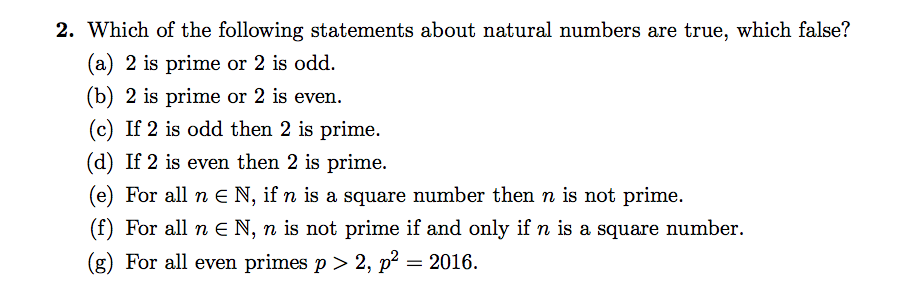
\includegraphics[width=450pt]{img/iulm-2-2.png}
\begin{mdframed}
  \begin{enumerate}[(a)]
  \item 2 is prime or 2 is odd.\\
    True. 2 is prime.
  \item 2 is prime or 2 is even.\\
    True. 2 is prime.
  \item If 2 is odd then 2 is prime.\\
    True. Premise is false so implication is true for all values of conclusion.
  \item If 2 is even then 2 is prime.\\
    True. Premise is true and conclusion is true, so implication is true.
  \item For all $n \in \N$, if $n$ is a square number then $n$ is not prime.\\
    False, 1 is a square number yet not prime.
  \item For all $n \in \N$, $n$ is not prime if and only if $n$ is a square number.\\
    False. 6 is not prime and yet not a square number.
  \item For all even primes $p > 2$, $p^2 = 2016$.\\
    True. There are no even primes greater than 2;
    $\forall ~ x \in \emptyset, ~p(x)$ is true for any predicate $p$.
  \end{enumerate}
\end{mdframed}


\subsection*{}
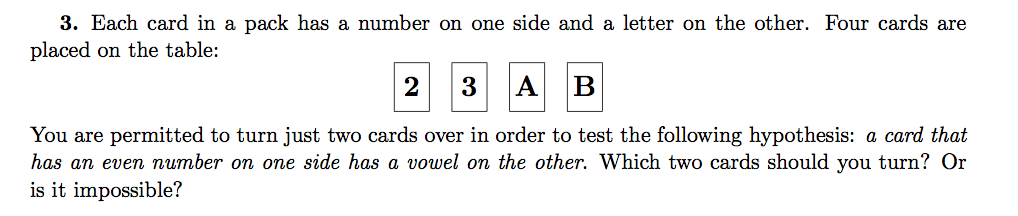
\includegraphics[width=450pt]{img/iulm-2-3.png}
\begin{mdframed}
  I think the wording of this question is ambiguous: ``A card that has an even
  number on one side has a vowel on the other'' might mean either of the
  following:
\begin{enumerate}
\item $\exists ~ c: \text{even}(c) \text{~and~} \text{vowel}(c)$
\item $\text{even}(c) \implies \text{vowel}(c)$.
\end{enumerate}
If we assume the intended meaning is (2), then we could disprove the hypothesis
by finding an even card with a consonant. So we could try cards 2 and B. That
might lead to a counter-example. If it does not, then the experiment is
inconclusive, because a counter-example may exist in the unavailable cards in
the rest of the pack.

If we assume the intended meaning is (1), then we could try turning over 2 and
A. That might lead to an example confirming the truth of the hypothesis. If it
does not, then the experiment is inconclusive, because a confirmation may exist
in the unavailable cards in the rest of the pack.
\end{mdframed}

\subsection*{}
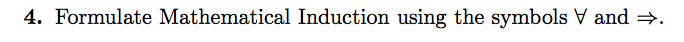
\includegraphics[width=400pt]{img/iulm-2-4.png}
\begin{mdframed}
\subsubsection*{Mathematical induction}
Consider a predicate function $p: \N \to \{\text{true},\text{false}\}$. We want to show
that $p(i)$ is true for all $i \in N$. In other words,

\textbf{Proposition}: $\forall ~ i \in N ~ p(i)$.\\

\textbf{Proof by induction}: First demonstrate that $p(0)$ is true. Next,
demonstrate that $p(i) \implies p(i+1)$.

\end{mdframed}

\subsection*{}
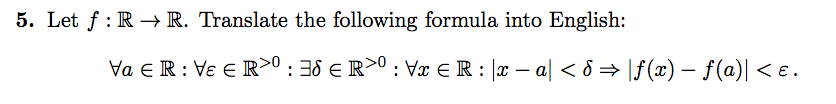
\includegraphics[width=400pt]{img/iulm-5.png}
\begin{mdframed}
  For all real numbers $a$ and positive reals $\epsilon$, there exists a
  positive real $\delta$ for which the following is true: for all real numbers
  $x$, $f(x)$ lies within a distance $\epsilon$ of $f(a)$ whenever $x$ lies
  within a distance $\delta$ of $a$.
\end{mdframed}

\subsection*{}
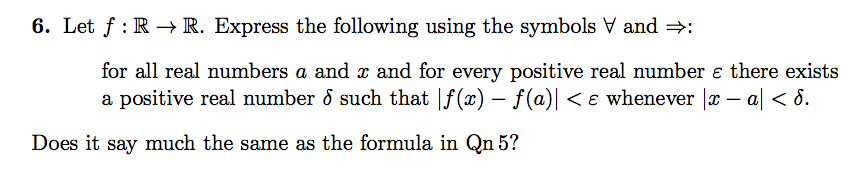
\includegraphics[width=400pt]{img/iulm-2-6.png}
\begin{mdframed}
  \begin{align*}
    \forall a \in \R: \forall x \in \R: \forall \epsilon \in \R^{>0}: \exists \delta \in \R^{>0}: |x - a| < \delta \implies |f(x) - f(a)| < \epsilon.
  \end{align*}
Yes it says much the same thing.
\end{mdframed}

\subsection*{}
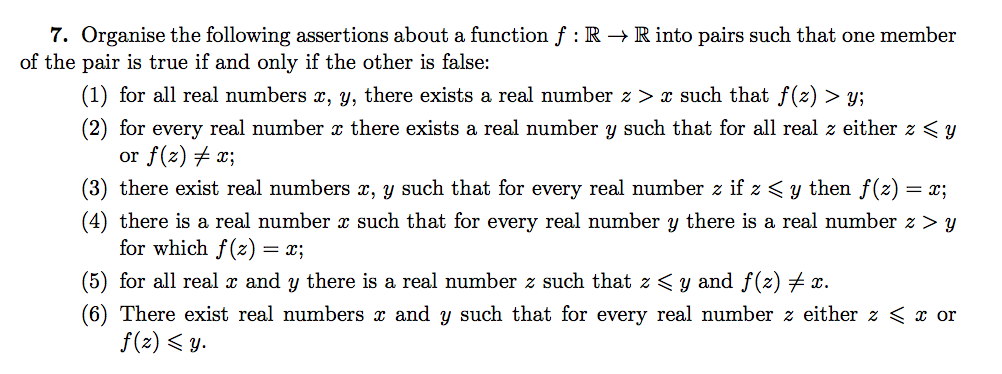
\includegraphics[width=450pt]{img/iulm-2-7.png}
\begin{mdframed}
  \begin{tabular}{c|c}
    1 &
  \end{tabular}
\end{mdframed}


\subsection*{}
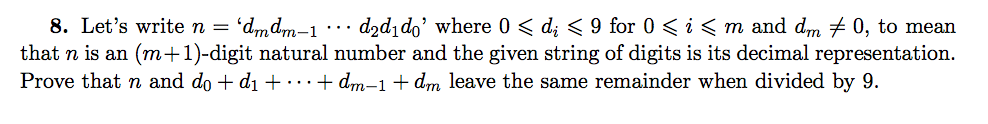
\includegraphics[width=450pt]{img/iulm-2-8.png}
\begin{mdframed}
  \subsubsection*{Proof}
  We have $n = \sum_{i=0}^m d_i 10^m$, and let $s(n) = \sum_{i=0}^m d_i$. Let
  $\bar{i}$ be the equivalence class of numbers that have $i \mod 9$ as their
  remainder when divided by 9 (clear way to make this definition?). The claim
  is that
  \begin{align*}
  \bar n = \bar{s(n)}.
  \end{align*}
  The key observation is that $\bar {10} = \bar 1$, so that the two summations
  expressions above end up mapping to the same equivalence class.

  To show this, note that the function that maps $i$ to $\bar i$ is a
  homomorphism, preserving both addition
  \begin{align*}
  \bar{i + j} = \bar i \oplus \bar j
  \end{align*}
  and multiplication
  \begin{align*}
  \bar{ij} = \bar i \otimes \bar j,
  \end{align*}
  where $\oplus$ and $\otimes$ denote the addition and multiplication
  operations on the set of equivalence classes. (The notation below doesn't
  always manage to distinguish between addition and multiplication on $\Z$
  versus the $\oplus$ and $\otimes$ operators.) Therefore
  \begin{align*}
    \bar n &= \bar{\sum_{i=0}^m d_i 10^m}
           = \sum_{i=0}^m \bar{d_i 10^m}
           = \sum_{i=0}^m \bar{d_i} \otimes \bar{10^m}
           = \sum_{i=0}^m \bar{d_i} \otimes \bar{10}~^m
           = \sum_{i=0}^m \bar{d_i} \otimes \bar{1}~^m\\
           &= \sum_{i=0}^m \bar{d_i} \otimes \bar{1}
           = \sum_{i=0}^m \bar{d_i}
           = \bar{\sum_{i=0}^m d_i} = \bar{s(n)}. \qed\\
  \end{align*}
  Alternatively,
  \begin{align*}
    n \mod 9 = s(n) \mod 9
    &\iff n - s(n) = 0 \mod 9\\
    &\iff \sum_{i=0}^m d_i 10^m - d_i = 0 \mod 9\\
    &\iff (10^m - 1)\sum_{i=0}^m d_i = 0 \mod 9\\
  \end{align*}
  which is true for all valid values of $m$ and $d_i$.
\end{mdframed}


\subsection*{}
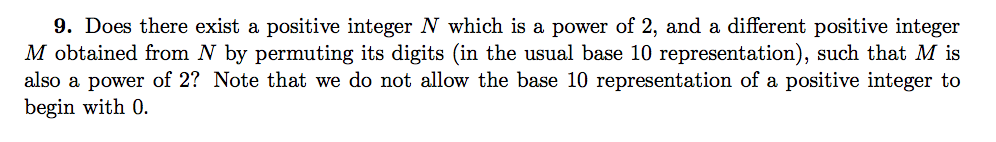
\includegraphics[width=450pt]{img/iulm-9.png}
\begin{mdframed}
  Not sure how to solve this, but here are a few observations:
  \begin{enumerate}
  \item If the two integers exist, they have the same number of digits in their
    decimal representation. I.e., they both lie in
    ${10^k,10^k + 2, \ldots, 10^{k+1} - 2}$ for some $k \geq 0$.
  \item For each ``order of magnitude'' $k$, there are either 3 or 4 powers of
    2.\footnote{To see this, note that we'll fit the most in if the first one
      is $10^k$ itself. (Powers of 2 are never actually a multiple of 10, but
      this will still give the upper bound.) Then
      $2\cdot 10^k, 2^2\cdot 10^k,2^3\cdot 10^k$ also fit in, giving
      4. Alternatively, the fewest that will fit in is when the first one is
      $2(10^k - 2)$. In this case we'll also get $2^2(10^k - 2)$ and
      $2^3(10^k - 2)$, giving 3.}
  \item We can re-phrase the question as follows:
    \begin{itemize}
    \item Visualize the powers of 2 belonging to the $k$-th order
      of magnitude as points in a $k$-dimensional grid with gridlines at
      $0, 1, 2, ...$. So for example, for $k=2$, the powers of 2 are
      $\{16, 32, 64\}$ and the points in the grid are
      $\{(1,6), (3,2), (6,4)\}$.
    \item Define an ``axis permutation'' of such a grid to be an operation that
      exchanges two of the coordinate axes, sending each occupied grid point to a
      new grid point.
    \item Define a ``congruent pair'' to be an ordered pair $(n_1, n_2)$ of
      powers of two, belonging to the same order of magnitude $k$, which has
      the following property: there exists some sequence of axis permutations
      after which the new location of $n_1$ is equal to the original location
      of $n_2$.
    \item Then we can rephrase the original question as: does there exist a $k$
      for which a congruent pair exists?
    \end{itemize}
  \end{enumerate}

  I looked up the proof:

  It's proof by contradiction. Suppose the pair of powers of 2 exist. The key
  observation is that we can use the mod 9 theorem: since the digits are the
  same (permuted) in the two integers, they sum to the same, and therefore the
  two integers are equal mod 9. Therefore their difference is a multiple of
  9. We know that the 4 values that are of the same length are $M, 2M, 4M,
  8M$. So if there's a pair that differ by permutation of their digits, then
  the difference between them must be $M, 3M$ or $7M$. In each case, that would
  mean that $M$ is a multiple of 9, and therefore not a power of 2. That
  contradiction proves it.

\end{mdframed}

\end{document}
